\lecture{Thu. 10/18/12}

Now that we've wrapped up the first half on computability theory, we have a midterm next Thursday, on the 3rd floor of Walker, at the usual time 11:00--12:30. It is open book (the book for this course only)/handouts/notes and covers everything through the last lecture. The test will contain about 4 problems.

Last time we talked about
\begin{itemize}
\item
the recursion theorem, and
\item
an introduction to logic.
\end{itemize}
Today we'll talk about
\begin{itemize}
\item
an introduction to complexity theory,
\item
TIME ($t(n)$), and
\item
$P$.
\end{itemize}

We're shifting gears to talk about complexity theory. Today we will introduce the subject and set up the basic model and definitions.
\subsection{Introduction to complexity theory}
We have to go slow at the beginning to get the framework clear. We'll begin by a simple example. In computability theory a typical question is whether a problem is decidable or not. As a research area that was mostly finished in the 50's. Now we'll restrict our attention to decidable languages. The question now becomes

\begin{center}
how many time or resources do we need to decide?
\end{center}

This has been an ongoing area of research since the 60's.

Let $A=\set{0^k1^k}{k\ge 0}$. This is a decidable language (in fact, context-free). We want to know how hard it is to see whether a string is in $A$. We could measure hardness in terms of number of steps, but the number of steps depend on the input. For longer strings it may take more time, and within strings of same length, some strings may take longer than others. For instance, if the string starts with 1, we can reject immediately. The picture is a bit messy, so to simplify, we'll only consider (other do diff things), we'll only consider how much time is necessary as a function of the length $n$ of the input.  %$N$ will always mean the length of the input. 
Among all inputs of given length, we'll try to determine what the worst case is, that is, we consider the worst case complexity. %some people average

Summarizing, we consider how the number of Turing machine steps depends on the input length $n$, and look at the worst case.

Recall that no matter whether we considered single tape, multi-tape, or nondeterministic Turing machines, what is computable remains invariant. This is not true for complexity theory: The picture will change depending on what model you use. 

We're not seeking to develop a theory of one-tape Turing machines. Turing machines are a stand-in for computation. We want to try to understand computation. What can do in principle, in a reasonable amount of time? We don't want to just focus on Turing machines.

The fact that complexity depends on the model is a problem. Which should we pick? But as we will see, although it depends on model, it doesn't depend {\it too much}, and we {\it can} recover useful theorems.

\subsubsection{An example}

\begin{ex}
We analyze how much space it takes to decide $A=\set{0^k1^k}{k\ge 0}$.

Let $M_1$=``(1-tape Turing machine) 
\begin{enumerate}
\item
Scan the input to test whether $w\in 0^*1^*$. We'll make a pass over the input just to see it's of the right form: no 1's before 0's. %finite automata.
\item Go back to the beginning. Mark off 0 (turn it into another symbol), mark off a 1, then go back to mark off the next 0, then the next 1, and so forth. Continue until we run out of 0's, 1's, or both. If we run out of 0's or 1's first, then reject. If they run out at the same time, accept.

(We needed to spell this out to know how much time the machine is using.)

\begin{center}
\begin{figure}[h!]
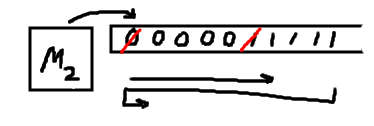
\includegraphics[scale=1.0]{12-1}
\qquad
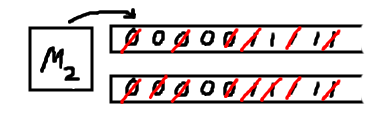
\includegraphics[scale=1.0]{12-2}
\end{figure}
\end{center}

In summary, repeat until all symbols are crossed off:
\begin{enumerate}
\item
Pass over input, cross off 0's and 1's.
\item
If either finishes before other, \ul{reject}.
\end{enumerate}
\item If all symbols are crossed off, \ul{accept}.
\end{enumerate}
For this course, we won't care about the constant factors in the time used: $10n^2$ steps and $20n^2$ are equivalent for us. (We could have the machine do some work on the reverse, but we won't bother.)

How much time does $M_1$ take?
\end{ex}
\begin{thm}
A 1-tape Turing machine can decide $A$ using $cn^2$ steps for all inputs of length $n$ and some fixed constant $c$. 
\end{thm}
We specify number of steps up to constants, so it's convenient to have notation for this. 
We'll refer to $cn^2$ as $O(n^2)$. This means at most a constant times $n^2$, where the constant is independent of $n$.

The definition is spelled out in the book; see the definition there.
\begin{proof}
Construct $M_1$ is above. How long does each step take?
\begin{enumerate}
\item
Scan input to test $w\in 0^*1^*$. \fixme{This takes $O(n)$ time: $n$ steps to go forward and $n$ steps to go back.}%finite automata.
\item 
Repeat until all symbols are crossed off: \fixme{We need at most $\fc n2$ steps.}
\begin{enumerate}
\item
Pass over input, cross off 0's and 1's. \fixme{This takes $O(n)$ time.}
\item
If either finishes before other, \ul{reject}.
\end{enumerate}
\item If all crossed off, \ul{accept}.
\end{enumerate}
Thus $M_1$ takes time 
\[O(n)+\fc n2O(n)=O(n^2).\]
(the nice thing about $O$ notation is that we only have to look at the dominant term when adding. We can throw away smaller terms because we can absorb them into the constant in the  dominant term.)
\end{proof}
Is this possible, or can we do better? Let's still stick to one-tape Turing machine. This is not the best algorithm out there; we can find a better one. Here is a suggestion. Zigzagging over the input costs us a lot more time. What if we cross off more 0's and 1's on a pass? We can cross of two 0's and 1's, so this takes half as much time. But we ignore the constant factor, so for our purposes this isn't really an improvement.

We don't ignore these improvements not because they're unimportant. %: real-world problem. 
In the real world, it's good to save factor of 2, that's good. However, we choose to ignore these questions because we are looking at a different realm: questions that don't depend on constant factors, or even larger variations.

By ignoring some things, other things come out more visibly. %Like biologists, everything reduces to quarks. But looking at quarks not beneficial to study. 
For example, everything reduces to quarks, but it would not benefit biologists to study everything on the level of quarks.

\subsubsection{An improvement}
We {\it can} improve running time to $O(n\log n)$; this is significant from our standpoint. 
Instead of crossing out a fixed number of 0's and 1's, we'll cross off every other 0 and every other 1 (Fig. 2), remember the even/odd parity of the number of 0's and 1's, and makes sure the parities agree at every pass. 
%odd number odd number.
After every step we go to the beginning and repeat, but we ignore the crossed off symbols. We always check the parity at each step. If they ever disagree, which can only happen if the number of 0's and 1's are different, we reject. If the parity is the same at each step, then there must be same number of 0's as 1's. 
This is because the parities are giving the representation of number of symbols in binary (details omitted). %Even odd, odd, comes from $5=101_2$.

This is a more efficient algorithm but less obvious than the original algorithm. It looks like room there is room for improvement, because we only need $n$ steps to read the input. Could the algorithm do $O(n)$?

We can do $O(n)$ with 2 tapes as follows. Read across the 0's, and copy them onto the 2nd tape. Then read 1's on the 1st tape and match the 0's against the 1's on the second tape. We don't need to zigzag, and we can finish in $2n$ steps.

%impossible
%where counter. fixed tape alphabet.
%counter binary number. drag along with you. But counter grow logarithmically. Cost of dragging logarithmically costs n\log n steps. 
In fact there is a theorem that we cannot decide $A$ in $O(n)$ steps with a 1-tape Turing machine. If we can do a problem with $O(n)$ steps on a 1-tape Turing machine, then it is a regular language! (This is not obvious.) If the machine can only use order $n$ time, then the only thing it can do is regular languages: the ability to write doesn't help. %Maybe carrying along counter can be done efficiently. Reading back what you've written take beyond order $n$ in general. Nice analysis but not that easy to order.

%just restricting time complexity to linear time should force just to do regular lang. not obvious.
In fact, anything that takes time $o(n\log n)$ %little o
% less than $o(n\log n)$ gives 
must be a regular language as well. 

\subsection{Time Complexity: formal definition}
Which model should we pick to see how much time it takes?
In computability theory we had {\it model independence}, the Church-Turing Thesis. Any model that we pick captures the same class of languages.
Unfortunately, in complexity theory we have {\it model dependence}. Fortunately, for reasonable models, the dependence is not very big. Some interesting questions don't depend (much) on the choice of ``reasonable"  models.

In the meantime, we'll fix a particular model, set things up using that model, and show things don't change too much if we choose a different model. For convenience we'll choose the same model we had all along, a 1-tape Turing machine, then show that it doesn't change too much for other models.

\begin{df}
For $t:\N\to \N$, we say a Turing machine $M$ runs in time $t(n)$ if for all inputs $w$ of length $n$, $M$ on $w$ halts in at most $t(n)$ steps. 
\end{df}
For instance, we say $M$ runs in $n^2$ time if $M$ always halts in $n^2$ steps when we give it an input of length $n$.

We now define the class of languages we can do in a certain number of steps. 
\begin{df}
Define 
\[{\text{TIME}(t(n))}:=\set{A}{\text{some TM decides $A$ and runs in $O(t(n))$ times}}.\]
This is called a \textbf{time complexity class}.
\end{df}
%Fig.3. \fixme{All problems solved by Turing machine which takes time on the order of at most $\text{TIME}(n^2)$; it contains $\{0^k1^k\}$. $\text{TIME}(n\log n)$ is inside, contatins too. $\text{TIME}(n)$ doesn't contain.}
\ig{12-3}{1}

We defined the time complexity using 1-tape turing machines. For a 2-tape TM, what is in the classes could change. 
Once we draw the picture, we can ask: is there a language we can do in $n^2$ time but can't do in $n\log n$ time? We'll look at questions like this later on, and be able to answer of them.

\subsubsection{Polynomial equivalence}
Even though the theory depends on model, it doesn't depend too much. %I'll show you why. 
This comes from the following statement.
\begin{thm}%t time bound. enough time look at input. 
Let $t(n)\ge n$. Then every multi-tape TM $M$ that runs in $t(n)$ time has an equivalent 1-tape Turing machine $S$ that runs in order $O(t^2(n))$ time.
\end{thm}
In other words, converting a multi-tape TM to a single tape TM can only blow up the amount of time by squaring; the single tape TM can polynomially simulate the multi-tape TM.

You might think this is bad, but for a computer, this is not too bad. It could be worse (exponential).

%Polynomial simulation.

\begin{proof}
We analyze the standard simulation (from the proof of Theorem~\ref{thm:ntm}).

The conversion only ends up squaring the amount of time used. Indeed, it took the tapes and wrote them down next to each other on the tape. Every time the multitape machine $M$ did one step, the single-tape machine $S$ had to do a lot of steps, and then do an update. One step of $M$ might have $S$ pass over entire portion of tape. {\it Each tape can be at most $t(n)$ symbols long, because there are only $t(n)$ steps where it can write symbols.} There are a constant number of tapes. {\it Thus one pass at most $O(t(n))$ steps. The machine has make at most $t(n)$ passes. Thus the order is $O(t(n)^2)$.}

\ig{12-4}{1}
\end{proof}
Here is an informal definition.
\begin{df}
Two computational models are \textbf{polynomially equivalent} if each can simulate the other with at most polynomial increase ($t(n)$ can go to $O(t(n)^k)$ for some $k$).
\end{df}
All reasonable deterministic models of computation turn out to be polynomially equivalent. This is the complexity analogue of the Church-Turing Thesis. 
\begin{ax}[Church-Turing Thesis]\llabel{church-turing-complexity}
All reasonable deterministic models are polynomially equivalent.
\end{ax}
This includes one-tape TM's, multi-tape TM's, 2-dimensional TM's, and random access machines (which are closer to a real computer) which can write an index and grab the memory cell at that location (the address).

A real computer is a messy thing to discuss mathematically. It doesn't have infinite amount of memory. From some points of view, it is like a finite automaton. The most useful way to abstractify it is as a random access machine(RAM) or a parallel RAM (PRAM). If the machine only has polynomial parallism, then it is also polynomially equivalent.
%Depends on how much parallelism. If exponential parallelism, no. %exp 
%Polynomial parallelism, obviously equivalent.

The analogous question with nondeterministic TM's is hard. No one knows a polynomial simulation. It is a famous open problem whether we convert a nondeterministic TM to a deterministic TM with a polynomial increase in time.

\subsubsection{P}

The complexity version of the Church-Turing Thesis~\ref{church-turing-complexity} tells us the following.\\

\cpbox{
All reasonable deterministic models are polynomially equivalent. Thus, if we ignore polynomial differences, we can recover a complexity class independent of the model. 
}
\vskip0.15in
\begin{df}
Let 
\[
P=\bigcup_k \text{TIME}(n^k)=\text{TIME}(\text{poly}(n)).
\]
\end{df}
%n log n
%upper bounds
%within that time. If can do faster, can still do within that time. ex. n log n, might as well put n instead, not look at smaller possible factors. Replace n's get poly.
In other words, $P$ consists of all languages solvable in $O(n^k)$ time for some $k$.
%take union over all, get $P$.
Why is $P$ important? 
\begin{enumerate}
\item
The class $P$ is invariant under choice of reasonable deterministic model. Time classes change when we go from 1-tape to multi-tape TM's. But by using polynomial equivalence---taking the union over all $O(n^k)$---the class $P$ is not going to change from model to model. We get the same class $P$.

Mathematically speaking, this invariance is natural. $P$ not a class to do with Turing machines. It's to do with the \emph{nature of computation}.
\item
Polynomial time computability roughly corresponds to \emph{practical computability}.  %n^{100} algs rare.
It is a good litmus test: a good way of capturing what it means for a problem to be solvable practically.

Of course, practicality depends on context. There is a continuum between practical and unpractical algorithms, but polynomial computability is a good dividing line. 
\end{enumerate}
One feature of $P$ makes it mathematically nice, and one feature tell you something practical to real world. A math notion with both these aspects is very good.

This is why $P$ is such an influential notion in complexity theory and throughout math.

\subsubsection{Examples}
Let's look at something we can solve in polynomial time. 
Let 
\[
\text{PATH}=\set{\an{G,s,t}}{G\text{ is a directed graph with a path from $s$ to $t$}}.
\]
\begin{thm}
PATH$\in P$.
\end{thm}
The way to prove something like this is to give an algorithm that runs in polynomial time.
%clear can check right form in p time
\begin{proof}
``One input $\an{G,s,t}$,
\begin{enumerate}
\item
Mark a node $s$.\\
Repeat until nothing new is marked:
\begin{itemize}
\item
Mark any node pointed to by previously a marked node.
\end{itemize}
\item
\ul{Accept} if $t$ is marked and \ul{reject} if not.
\end{enumerate}
\end{proof}
\ig{12-5}{1}

We start at $s$, mark everything we can get to in 1 step by marking nodes adjacent to $s$; then we mark nodes adjacent to \emph{those}... This is a simple breadth-first search, not the best, but it runs in polynomial time.

We will often omit time analyses unless it is not obvious.
If each step runs in polynomial time, and all repetitions involve a  polynomial number of repeats, then the problem is solvable in $P$.

If we look at a similar problem, however, everything changes.

\begin{df}
A \textbf{Hamiltonian path} goes through every node exactly once.
\end{df}
%longest possible simple path that hits every node once. has to visit everything along the way.
%just knowing path doesn't tell you if there's a Hamiltonian path. Maybe path, but don't know if H path.
Is $\text{HAMPATH}\in P$? The algorithm above doesn't answer this question. It's a decidable problem because we can try every possible path, but there can be an exponential number of paths (in terms of the size of the graph).

The answer is not known! This is a very famous unsolved problem. 
